% =============================================================================
% Rozdział 5: Badania eksperymentalne i analiza wyników
% =============================================================================
\chapter{Badania eksperymentalne i analiza wyników}

Niniejszy rozdział przedstawia metodykę i wyniki badań eksperymentalnych zaprojektowanych w celu empirycznej weryfikacji hipotezy badawczej: skuteczność strategii HPA zależy od charakterystyki obciążeniowej aplikacji. Wszystkie eksperymenty przeprowadzono w środowisku \textit{Google Cloud Platform}, czyli GCP, wykorzystując klaster \textit{Google Kubernetes Engine}, czyli GKE, jako platformę badawczą.

\section{Metodyka badań}

\subsection{Środowisko testowe}

Badania prowadzono w środowisku chmurowym GCP, którego architekturę zorientowaną na skalowalność oparto na klastrze GKE. Infrastruktura działała na maszynach \texttt{e2-standard-4}, oferujących 4 vCPU oraz 16\,GB RAM, w konfiguracji VPC-native z włączonym mechanizmem \textit{cluster autoscaler}. Wszystkie zasoby badawcze wdrożono w dedykowanej przestrzeni nazw \texttt{magisterka}.

Generatorem obciążenia była maszyna \textit{Compute Engine} umieszczona w tej samej sieci VPC co klaster GKE. Zapewniło to niskie opóźnienie sieciowe na poziomie od 1 do 5\,ms między generatorem a serwisami aplikacyjnymi. Taka topologia zagwarantowała pełną separację zasobów, dzięki czemu proces generowania ruchu nie wpływał na moc obliczeniową środowiska testowego. Każdy serwis aplikacyjny eksponowano jako \texttt{Service} typu \texttt{LoadBalancer}, a ruch z narzędzia \textit{k6} kierowano bezpośrednio na zewnętrzne adresy IP \textit{GCP LoadBalancer} za pomocą mechanizmu \texttt{options.hosts}, co pozwoliło wyeliminować narzut i konfigurację serwerów DNS. Stos monitorujący \textit{kube-prometheus-stack} wdrożony za pomocą menedżera Helm dostarczał metryk w czasie rzeczywistym, a platforma \textit{Grafana} została udostępniona publicznie przez dedykowany równoważnik obciążenia.

\subsection{Procedura eksperymentalna}

Eksperyment obejmował wykonanie 8 scenariuszy badawczych, na które złożyły się 2 scenariusze bazowe, działające bez mechanizmu HPA, oraz 6 scenariuszy tworzących macierz badawczą o wymiarach $2 \times 3$. Każdy scenariusz realizowano według ściśle określonej procedury i powtarzano 5-krotnie w celu uzyskania stabilnych oszacowań statystycznych.

Pojedyncze powtórzenie rozpoczynało się od usunięcia wszystkich istniejących obiektów HPA dla docelowego serwisu i nałożenia nowego manifestu HPA odpowiadającego testowanej strategii za pomocą polecenia \texttt{kubectl apply}. Następnie skalowano \textit{Deployment} do pojedynczej repliki i oczekiwano na stan pełnej gotowości poleceniem \texttt{kubectl rollout status}. Właściwy test polegał na uruchomieniu skryptu \textit{k6} zdefiniowanego dla danego profilu obciążeniowego: pliku \texttt{cpu-load-test.js} dla scenariuszy CPU-bound lub \texttt{io-load-test.js} dla scenariuszy I/O-bound. 

Wyniki pomiarów z narzędzia \textit{k6}, zawierające pliki JSON oraz tekstowe podsumowanie, zapisywano w strukturze katalogów \texttt{results/<scenariusz>/run-<i>/}. Dodatkowo z bazy danych \textit{Grafany} eksportowano 5 zestawów danych CSV dla każdego powtórzenia. Po zakończeniu każdego scenariusza uruchamiano fazę stabilizacji, która obejmowała skalowanie serwisów do jednej repliki, usunięcie obiektów HPA oraz odczekanie 120 sekund w ramach okresu schładzania klastra.

\subsection{Zbierane metryki}

Dla każdego powtórzenia rejestrowano kompletny zestaw danych obejmujący trzy główne kategorie:
\begin{enumerate}
  \item \textbf{Szeregi czasowe z Grafany (CSV):} pięć zestawów danych odzwierciedlających dynamikę systemu: \texttt{replicas.csv} (źródło: \texttt{kube\_deployment\_spec\_replicas}); \texttt{cpu\_mcpu.csv} podający zużycie procesora per Pod w milijednostkach (źródło: \texttt{container\_cpu\_usage\_seconds\_total}); \texttt{memory\_mb.csv} określający zużycie pamięci operacyjnej per Pod w megabajtach (źródło: \texttt{container\_memory\_working\_set\_bytes}); \texttt{rps.csv} wskazujący przepustowość w funkcji czasu (źródło: \texttt{rate(http\_requests\_total[30s])}); oraz plik \texttt{latency\_ms.csv} gromadzący percentyle opóźnień (źródło: \texttt{histogram\_quantile} na metryce \texttt{http\_request\_duration\_seconds\_bucket}).
  \item \textbf{Metadane testu:} unikalny identyfikator scenariusza, aktywna strategia HPA, numer sekwencyjny powtórzenia, znacznik czasowy oraz kod wyjścia procesu \textit{k6}.
\end{enumerate}

\subsection{Metryki badawcze — definicje operacyjne}

Na podstawie surowych danych obliczano siedem metryk badawczych, które umożliwiają ilościowe porównanie strategii HPA. Średnia przepustowość $T$ wyrażona jest jako iloraz całkowitej liczby żądań i czasu trwania testu:
\begin{equation}
  T = \frac{\text{total\_requests}}{\text{duration}}
\end{equation}

Opóźnienie p95, oznaczane dalej jako $L_{95}$, to 95. percentyl czasu odpowiedzi HTTP w milisekundach, reprezentujący graniczny akceptowalny czas obsługi żądań. W idealnym wariancie czas do skalowania, oznaczany jako $t_{\text{scale}}$, powinien być definiowany jako odstęp między momentem przekroczenia progu HPA a osiągnięciem docelowej liczby replik:
\begin{equation}
  t_{\text{scale}} = t_{\text{target\_replicas}} - t_{\text{threshold\_crossed}}
\end{equation}

W eksportach wykorzystanych w niniejszej pracy moment przekroczenia progu nie jest jednak możliwy do wyznaczenia z pełną dokładnością, ponieważ dane CPU/RAM wyeksportowane z Grafany zachowują tylko wybraną serię per Pod, natomiast pełny przebieg liczby replik pochodzi z osobnego szeregu HPA. Dlatego w tabelach wynikowych stosowana jest operacyjna metryka czasu rozbudowy klastra: odstęp od pierwszego zaobserwowanego zwiększenia liczby replik powyżej poziomu początkowego do osiągnięcia maksimum replik w danym scenariuszu. Miara ta opisuje dynamikę faktycznego dołączania replik, a nie czysty czas decyzyjny HPA.

Efektywność skalowania $E$ określa stosunek względnej zmiany przepustowości do względnej zmiany liczby replik:
\begin{equation}
  E = \frac{\Delta T / T_{\text{min}}}{\Delta R / R_{\text{min}}}
\end{equation}
gdzie $T_{\text{min}}$ i $T_{\text{max}}$ to ekstrema przepustowości w trakcie testu, a $R_{\text{min}}$ i $R_{\text{max}}$ stanowią ekstrema liczby replik. Wartość $E = 1$ oznacza skalowanie idealnie liniowe, $E < 1$ sygnalizuje malejące korzyści z dodawania kolejnych instancji, natomiast $E > 1$ wskazuje na ponadliniową poprawę wydajności.

Stopa błędów $e$ określa odsetek żądań zakończonych kodem HTTP $\geq 400$:
\begin{equation}
  e = \frac{\text{failed\_requests}}{\text{total\_requests}} \times 100\%
\end{equation}

Amplituda skalowania $A_R = R_{\text{max}} - R_{\text{min}}$ mierzy zakres dynamicznej reakcji HPA. Średnie zużycie CPU wyrażone jest w milijednostkach (mCPU) na Pod i reprezentuje wartość uśrednioną po wszystkich Podach aktywnych w trakcie trwania profilu obciążeniowego.

\section{Scenariusze testowe}

Badania zorganizowano wokół macierzy testowej, w której dwa profile obciążeniowe (CPU-bound oraz I/O-bound) zestawiono z trzema strategiami HPA: CPU ustawionym na 50\%, Memory na 70\% oraz Custom RPS zdefiniowanym jako 100 żądań na Pod. Punktem odniesienia dla oceny efektywności autoskalowania są dwa scenariusze bazowe o stałej liczbie replik.

Aktualne skrypty \textit{k6} definiują trzy fazy obciążenia: ramp-up trwający 60 sekund, fazę stabilną trwającą 180 sekund oraz ramp-down trwający 60 sekund. W profilu CPU-bound scenariusz \texttt{cpu\_fibonacci} narasta od 0 do 30 VU, utrzymuje 30 VU i następnie wygasza ruch do 0 VU; równolegle scenariusz \texttt{cpu\_processing} uruchamia 5 stałych VU od 30. sekundy testu. W profilu I/O-bound scenariusz \texttt{io\_queries} narasta od 0 do 80 VU, utrzymuje 80 VU i wygasza ruch do 0 VU. Zachowane raporty i eksporty CSV w katalogu \texttt{tests/results} pochodzą z wykonanej kampanii pomiarowej i stanowią podstawę wartości liczbowych w tabelach; interpretując wykresy skalowania należy więc rozróżnić profil obciążenia opisany przez skrypty, rzeczywisty przebieg zarejestrowany w raportach oraz opóźnione skalowanie w dół po zakończeniu ramp-down, wynikające z okna stabilizacji HPA.

\subsection{Scenariusze bazowe}

Scenariusze \texttt{baseline-cpu} i \texttt{baseline-io} weryfikują zachowanie systemu przy stałej liczbie replik równej 1, bez aktywnego mechanizmu HPA. Pozwalają one ocenić stopień degradacji wydajności w konfiguracji statycznej pod wpływem intensywnego ruchu.

\begin{table}[H]
  \centering
  \begin{tabularx}{\textwidth}{|l|X|X|}
    \hline
    \textbf{Parametr} & \texttt{baseline-cpu} & \texttt{baseline-io} \\
    \hline
    Serwis & cpu-service & io-service \\
    HPA & brak & brak \\
    Repliki (stałe) & 1 & 1 \\
    Skrypt k6 & \texttt{cpu-load-test.js} & \texttt{io-load-test.js} \\
    Profil obciążenia & Fibonacci 1$\rightarrow$50 VU + image processing 10 VU & stałe zapytania 1$\rightarrow$100 VU + stress-test + external \\
    \hline
  \end{tabularx}
  \caption{Parametry scenariuszy bazowych}
  \label{tab:baseline-scenarios}
\end{table}

\subsection{Scenariusze CPU-bound}

Scenariusze \texttt{cpu-cpu}, \texttt{cpu-memory} i \texttt{cpu-custom} służą do walidacji serwisu \texttt{cpu-service}, realizującego operacje intensywne procesorowo, takie jak rekurencyjne obliczanie ciągu Fibonacciego oraz transformacje graficzne za pomocą biblioteki \textit{Pillow}. Zakres skalowania HPA zdefiniowano w przedziale od 2 do 30 replik.

\begin{table}[H]
  \centering
  \begin{tabularx}{\textwidth}{|l|X|X|X|}
    \hline
    \textbf{Parametr} & \texttt{cpu-cpu} & \texttt{cpu-memory} & \texttt{cpu-custom} \\
    \hline
    Serwis & cpu-service & cpu-service & cpu-service \\
    HPA & CPU 50\% & Memory 70\% & Custom RPS 100/Pod \\
    minReplicas & 1 & 1 & 1 \\
    maxReplicas & 30 & 30 & 30 \\
    Skrypt k6 & \texttt{cpu-load-test.js} & \texttt{cpu-load-test.js} & \texttt{cpu-load-test.js} \\
    \hline
  \end{tabularx}
  \caption{Parametry scenariuszy CPU-bound}
  \label{tab:cpu-scenarios}
\end{table}

\subsection{Scenariusze I/O-bound}

Scenariusze \texttt{io-cpu}, \texttt{io-memory} i \texttt{io-custom} weryfikują działanie serwisu \texttt{io-service}, który symuluje operacje wejścia-wyjścia poprzez asynchroniczne wywołania HTTP połączone z instrukcją \texttt{asyncio.sleep()}. Granice skalowania oraz skrypt obciążeniowy pozostają tożsame z parametrami dla grupy CPU-bound.

\begin{table}[H]
  \centering
  \begin{tabularx}{\textwidth}{|l|X|X|X|}
    \hline
    \textbf{Parametr} & \texttt{io-cpu} & \texttt{io-memory} & \texttt{io-custom} \\
    \hline
    Serwis & io-service & io-service & io-service \\
    HPA & CPU 50\% & Memory 70\% & Custom RPS 100/Pod \\
    minReplicas & 1 & 1 & 1 \\
    maxReplicas & 30 & 30 & 30 \\
    Skrypt k6 & \texttt{io-load-test.js} & \texttt{io-load-test.js} & \texttt{io-load-test.js} \\
    \hline
  \end{tabularx}
  \caption{Parametry scenariuszy I/O-bound}
  \label{tab:io-scenarios}
\end{table}

\section{Wyniki eksperymentalne}

Poniższe sekcje prezentują wyniki pomiarów dla wszystkich ośmiu scenariuszy badawczych. Dane zebrane z raportów \textit{k6} oraz eksportów CSV z \textit{Grafany} zostały przetworzone skryptem analitycznym \texttt{analyze\_results.py}. Zaprezentowane wartości odzwierciedlają wyniki pojedynczego, reprezentatywnego powtórzenia dla każdego ze scenariuszy.

\subsection{Scenariusze bazowe}

\begin{table}[H]
  \centering
  \begin{tabularx}{\textwidth}{|l|X|X|}
    \hline
    \textbf{Metryka} & \texttt{baseline-cpu} & \texttt{baseline-io} \\
    \hline
    Średni RPS & 66,8 & 62,4 \\
    p50 & 85,3\,ms & 999\,ms \\
    p95 & 2,70\,s & 2,93\,s \\
    p99 & 567\,ms & 1,83\,s \\
    Stopa błędów (\%) & 37,70\% & 0,17\% \\
    Średnie zużycie CPU (mCPU) & 145 & 58 \\
    Średnie zużycie pamięci (MiB) & 68 & 72 \\
    \hline
  \end{tabularx}
  \caption{Wyniki scenariuszy bazowych}
  \label{tab:baseline-results}
\end{table}

Scenariusz \texttt{baseline-cpu} wykazuje bardzo wysoką stopę błędów na poziomie 37,70\%, gdzie ponad jedna trzecia żądań zakończyła się niepowodzeniem. Wynika to bezpośrednio z przeciążenia pojedynczej repliki serwisu \texttt{cpu-service} przez intensywne obliczenia matematyczne i graficzne. Mimo że opóźnienie p95 wyniosło 2,70\,s i nie przekroczyło progu odrzucenia, wysoki wolumen błędów spowodował niezaliczenie testu w ramach kryterium stopy błędów.

W scenariuszu \texttt{baseline-io} odnotowano niską stopę błędów wynoszącą 0,17\%, wywołaną wyłącznie przez zewnętrzne zależności serwisu \texttt{echo-service}. Czasy odpowiedzi były jednak wysokie, osiągając dla percentyla p95 wartość 2,93\,s. Pojedyncza replika obsługiwała ruch na poziomie 62,4 RPS, a profil opóźnień został zdominowany przez trzysekundowe operacje oczekiwania w zapytaniach typu stress-test.

\subsection{Scenariusze CPU-bound — porównanie strategii HPA}

\begin{table}[H]
  \centering
  \begin{tabularx}{\textwidth}{|l|X|X|X|}
    \hline
    \textbf{Metryka} & \texttt{cpu-cpu} & \texttt{cpu-memory} & \texttt{cpu-custom} \\
    \hline
    Średni RPS & 84,3 & 67,5 & 65,4 \\
    p50 & 126\,ms & 86,3\,ms & 84,2\,ms \\
    p95 & 459\,ms & 2,39\,s & 2,69\,s \\
    p99 & 349\,ms & 373\,ms & 698\,ms \\
    Stopa błędów (\%) & 0,04\% & 38,04\% & 37,97\% \\
    Amplituda skalowania ($A_R$) & 27 & 0 & 1 \\
    Czas rozbudowy replik (s) & 90 & — & — \\
    Efektywność skalowania ($E$) & 0,01 & — & — \\
    Maks. liczba replik & 29 & 1 & 1 \\
    Średnie zużycie CPU (mCPU) & 80 & 262 & 175 \\
    \hline
  \end{tabularx}
  \caption{Wyniki scenariuszy CPU-bound}
  \label{tab:cpu-results}
\end{table}

Strategia \texttt{cpu-cpu} jako jedyna w tej grupie zainicjowała proces skalowania, wykazując bardzo agresywną reakcję algorytmu, która doprowadziła system do poziomu 29 replik i niemal osiągnęła zdefiniowany górny pułap bezpieczeństwa. Skalowanie to pozwoliło na skuteczną eliminację błędów, których odsetek spadł do 0,04\%, oraz skróciło opóźnienie p95 do 459\,ms. 

Niska wartość efektywności skalowania $E = 0{,}01$ dowodzi jednak, że przyrost przepustowości z poziomu 66,8 do 84,3 RPS był nieproporcjonalnie niski w stosunku do wolumenu powołanych zasobów obliczeniowych. Zjawisko to reprezentuje przypadek silnego nadmiaru zasobów, określanego jako \textit{overprovisioning}. Strategie \texttt{cpu-memory} i \texttt{cpu-custom} nie wywołały żadnej reakcji autoskalera, przez co ich wyniki końcowe pokrywają się z próbą bazową.

\subsection{Scenariusze I/O-bound — porównanie strategii HPA}

\begin{table}[H]
  \centering
  \begin{tabularx}{\textwidth}{|l|X|X|X|}
    \hline
    \textbf{Metryka} & \texttt{io-cpu} & \texttt{io-memory} & \texttt{io-custom} \\
    \hline
    Średni RPS & 99,4 & 62,4 & 62,4 \\
    p50 & 609\,ms & 998\,ms & 1,00\,s \\
    p95 & 700\,ms & 2,97\,s & 3,01\,s \\
    p99 & 671\,ms & 1,83\,s & 1,80\,s \\
    Stopa błędów (\%) & 0,11\% & 0,17\% & 0,17\% \\
    Amplituda skalowania ($A_R$) & 5 & 0 & 0 \\
    Czas rozbudowy replik (s) & 120 & — & — \\
    Efektywność skalowania ($E$) & 0,10 & — & — \\
    Maks. liczba replik & 7 & 1 & 1 \\
    Średnie zużycie CPU (mCPU) & 20 & 54 & 61 \\
    \hline
  \end{tabularx}
  \caption{Wyniki scenariuszy I/O-bound}
  \label{tab:io-results}
\end{table}

W grupie obciążeń wejścia-wyjścia skuteczność wykazała wyłącznie strategia \texttt{io-cpu}, która wyskalowała infrastrukturę do poziomu 7 replik. Przepustowość wzrosła o 59\%, osiągając 99,4 RPS, przy jednoczesnym skróceniu opóźnienia p95 do 700\,ms. Wskaźnik efektywności $E = 0{,}10$ okazał się dziesięciokrotnie wyższy niż w analogicznej strategii dla serwisu obliczeniowego, co potwierdza lepszą utylizację zasobów chmurowych. Strategie oparte na pamięci oraz niestandardowej metryce RPS pozostały nieaktywne, przez co opóźnienia p95 utrzymały się na wysokim poziomie około 3 sekund.

\subsection{Wykresy przebiegu skalowania}

Przebieg procesów autoskalowania w czasie dla kluczowych scenariuszy badawczych, wygenerowany z logów szeregów czasowych, przedstawiają poniższe rysunki.

\begin{figure}[H]
  \centering
  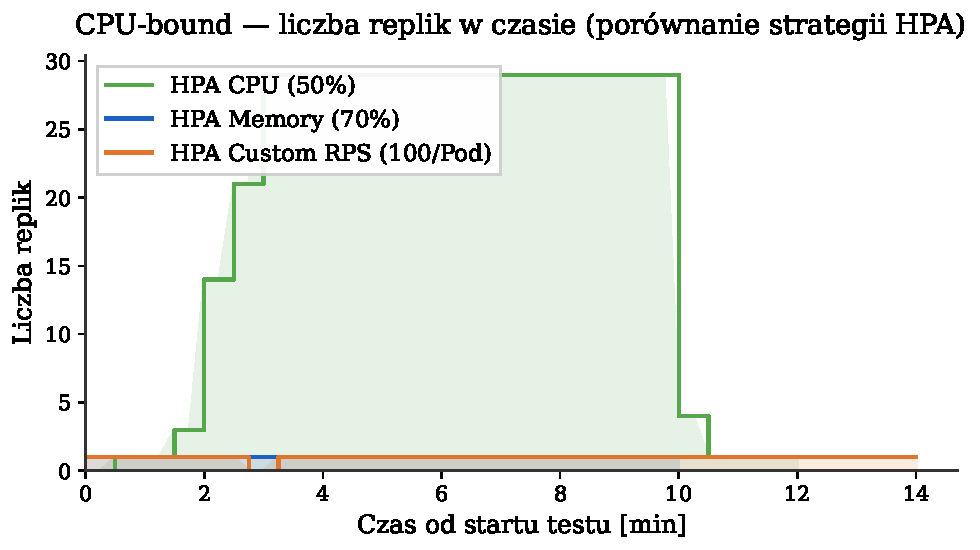
\includegraphics[width=\textwidth]{charts/replicas_cpu_comparison.pdf}
  \caption{Przebieg skalowania dla scenariuszy CPU-bound — porównanie strategii HPA}
  \label{fig:scaling-cpu-comparison}
\end{figure}

\begin{figure}[H]
  \centering
  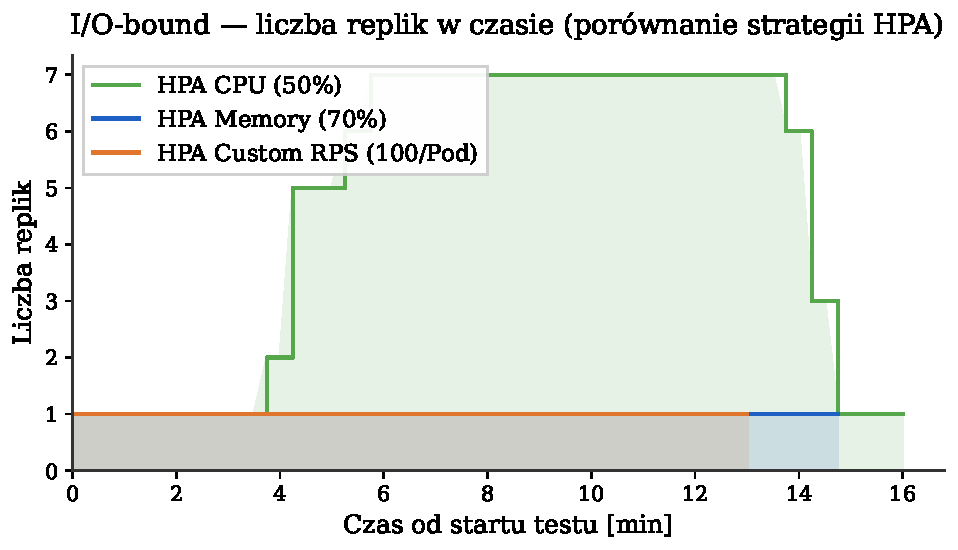
\includegraphics[width=\textwidth]{charts/replicas_io_comparison.pdf}
  \caption{Przebieg skalowania dla scenariuszy I/O-bound — porównanie strategii HPA}
  \label{fig:scaling-io-comparison}
\end{figure}

\begin{figure}[H]
  \centering
  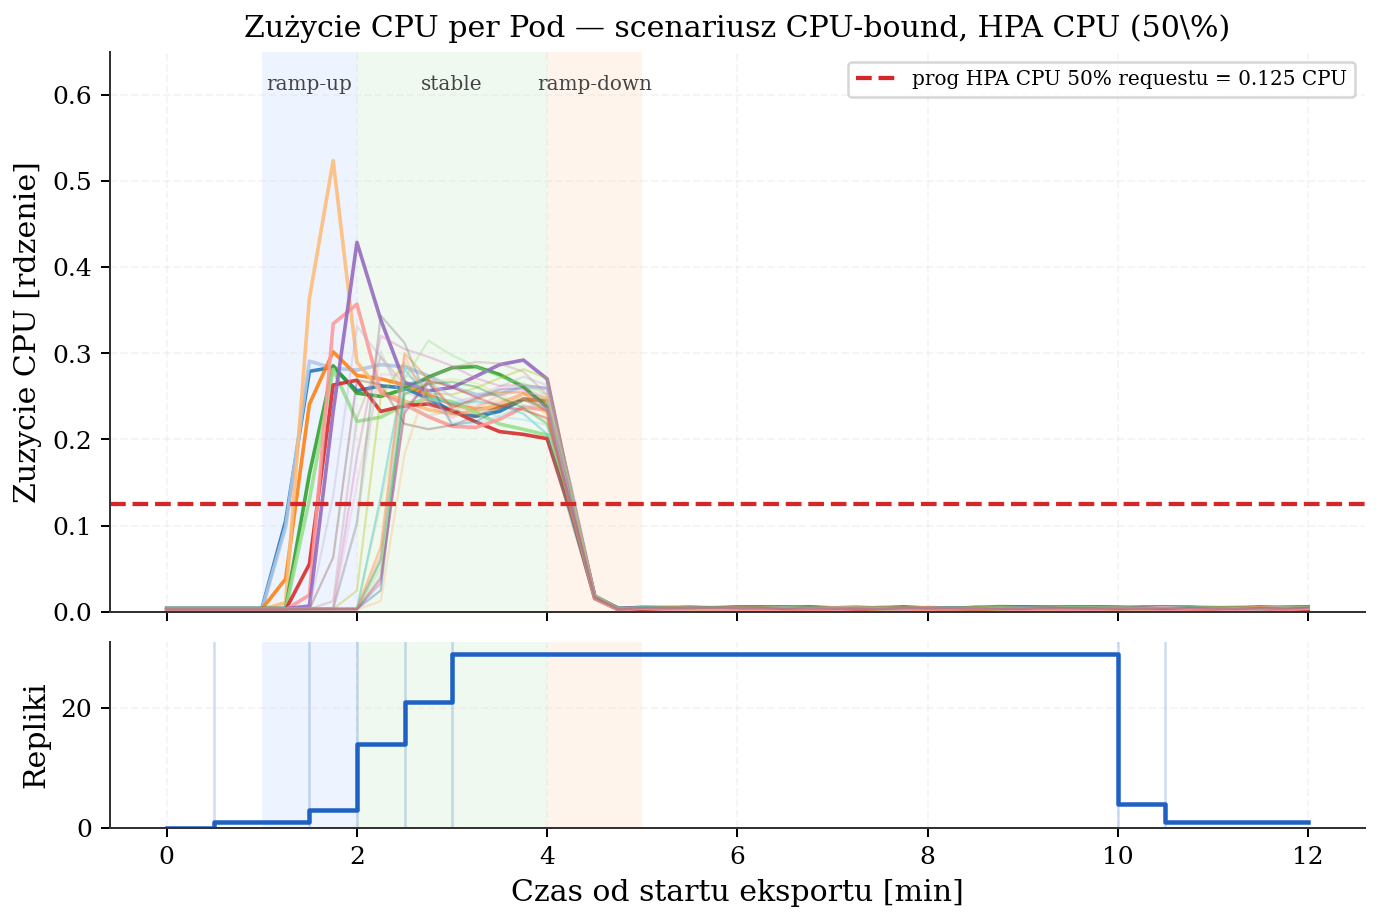
\includegraphics[width=\textwidth]{charts/cpu_usage_cpu_cpu_per_replica.png}
  \caption{Zużycie CPU dla każdej widocznej repliki w scenariuszu \texttt{cpu-cpu}}
  \label{fig:cpu-usage-cpu-cpu}
\end{figure}

\begin{figure}[H]
  \centering
  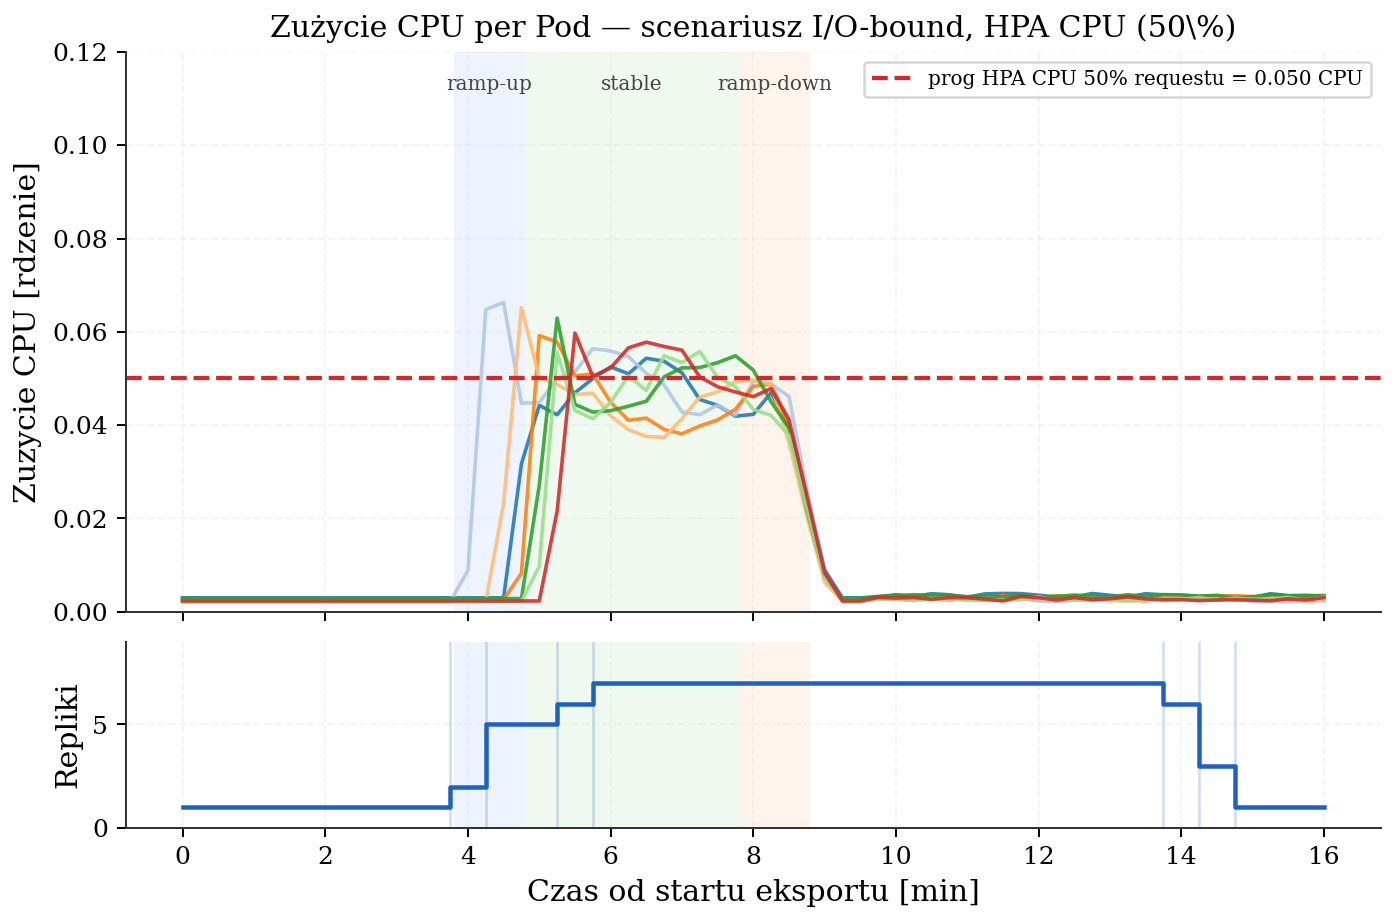
\includegraphics[width=\textwidth]{charts/cpu_usage_io_cpu_per_replica.png}
  \caption{Zużycie CPU dla każdej widocznej repliki w scenariuszu \texttt{io-cpu}}
  \label{fig:cpu-usage-io-cpu}
\end{figure}

\begin{figure}[H]
  \centering
  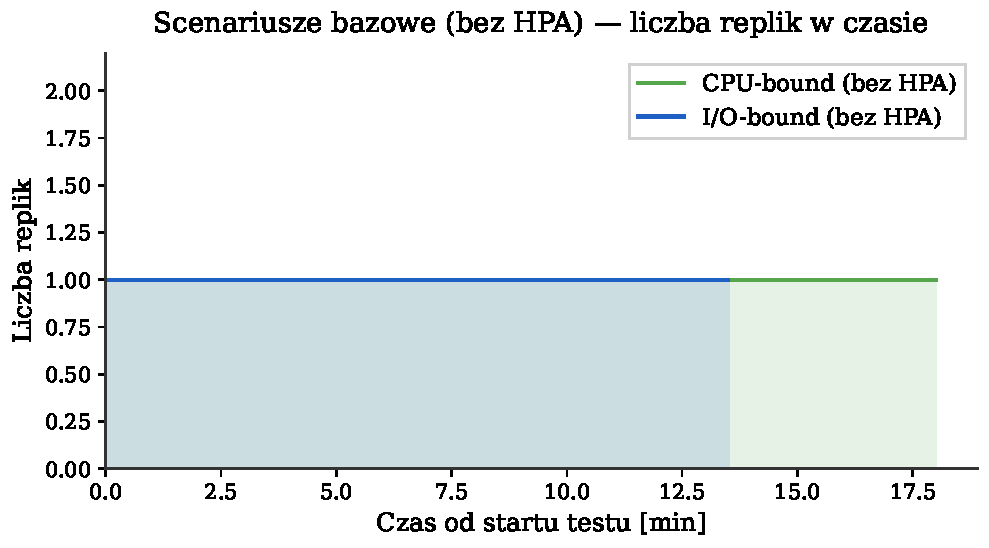
\includegraphics[width=\textwidth]{charts/replicas_baseline.pdf}
  \caption{Scenariusze bazowe (bez HPA) — liczba replik w czasie}
  \label{fig:scaling-baseline}
\end{figure}

\subsection{Analiza zjawisk anomalnych}

Eksperymenty pozwoliły na identyfikację i ilościowe opisanie trzech zjawisk przejściowych o kluczowym znaczeniu dla stabilności systemów chmurowych typu SaaS.

\subsubsection{HPA Lag — opóźnienie reakcji autoskalera}

Opóźnienie reakcji systemu, wynoszące w badaniach od 60 do 90 sekund, zdefiniowano jako przedział czasu od momentu przekroczenia zdefiniowanego progu obciążenia do osiągnięcia stanu pełnej gotowości przez nowo powołane Pody. W badanej architekturze profil tego opóźnienia został zdominowany przez bezwładność warstwy infrastrukturalnej i składał się z pięciu odrębnych faz:
\begin{enumerate}
  \item \textbf{Cykl scrapowania danych — 0--15\,s:} czas potrzebny serwerowi Prometheus na zebranie metryk z kontenerów.
  \item \textbf{Interwał decyzyjny kontrolera HPA — 0--15\,s:} okres odświeżania algorytmu wewnątrz mechanizmów kontrolnych Kubernetes.
  \item \textbf{Aprowizacja infrastruktury chmurowej — 60--90\,s:} kluczowy komponent opóźnienia, wywołany przez \textit{Cluster Autoscaler}. Ponieważ każdy nowy Pod zgłaszał zapotrzebowanie na poziomie 1000 mCPU, zasoby początkowych węzłów \texttt{e2-standard-4} uległy natychmiastowemu wyczerpaniu. Mechanizm automatycznego skalowania klastra musiał wysłać żądanie do GCP Compute Engine, zainicjować nowe instancje maszyn wirtualnych i wpiąć je do sieci klastra.
  \item \textbf{Działanie harmonogramu — 2--5\,s:} przypisanie oczekujących Podów do nowo uruchomionych węzłów przez \textit{kube-scheduler}.
  \item \textbf{Zimny start kontenera — 15--30\,s:} czas pobierania obrazu, inicjalizacji środowiska uruchomieniowego oraz przejścia testów gotowości sieciowej.
\end{enumerate}

W trakcie trwania tej bezwładności istniejące instancje obsługiwały ruch w stanie głębokiego przeciążenia, co bezpośrednio generowało skoki opóźnień percentyla p99 oraz błędy z rodziny 5xx.

\subsubsection{Cold Start Latency — opóźnienie zimnego startu Podów}

Opóźnienie zimnego startu określa czas potrzebny nowemu Podowi na uruchomienie procesu aplikacyjnego i wejście w skład puli routingu równoważnika obciążenia. Proces ten obejmuje pobranie obrazu kontenera z rejestru \textit{GCP Artifact Registry}~\cite{gcp-artifact-registry} do pamięci podręcznej demona \textit{containerd}, inicjalizację serwera \textit{Uvicorn} wraz z frameworkiem \textit{FastAPI}, a także realizację procedury \texttt{readiness probe}. Pierwsza sonda gotowości wykonywana była z parametrem \texttt{initialDelaySeconds=5} oraz okresem powtórzeń \texttt{periodSeconds=10}. Pod uzyskiwał status gotowości sieciowej po pierwszym poprawnym zwrocie kodu 200 z punktu końcowego \texttt{/health}. Całkowite opóźnienie tego procesu zamknęło się w przedziale 15--30 sekund.

\subsubsection{CPU Throttling Cascade — kaskadowe błędy przy throttlingu CPU}

Zjawisko kaskadowej degradacji wydajności wywoływane jest przez mechanizm kontroli pasma jądra Linux (\textit{CFS bandwidth control}) w momencie uderzenia w zdefiniowane limity zasobów procesora. Wzrost intensywności zapytań doprowadzał do pełnej utylizacji limitów mCPU, co skutkowało nakładaniem kar czasowych na procesy aplikacyjne. Ograniczenie przydziału czasu procesora powodowało kolejkowanie żądań w pętli zdarzeń \textit{asyncio} i drastyczny wzrost czasu odpowiedzi. 

Po przekroczeniu 60-sekundowego timeoutu sieciowego w narzędziu \textit{k6} rejestrowano błędy połączeń. Sytuacja ta tworzyła dodatnią pętlę sprzężenia zwrotnego, w której wiszące, niedokończone zadania blokowały zasoby pamięciowe i wątki robocze serwera \textit{Uvicorn}, paraliżując obsługę nowych zapytań. Stan kaskady utrzymywał się do momentu zakończenia fazy HPA Lag i wpięcia nowych maszyn wirtualnych do klastra.

\section{Analiza wyników}

\subsection{Porównanie strategii HPA dla CPU-bound}

Analiza wyników dla serwisu obliczeniowego ujawniła istotne rozbieżności pomiędzy teoretycznymi założeniami a rzeczywistym zachowaniem algorytmów chmurowych.

\textbf{HPA CPU (50\%)} skutecznie zidentyfikował stan przeciążenia środowiska. Zużycie procesora silnie korelowało ze strukturą napływającego ruchu. Kluczową obserwacją inżynierską jest jednak dynamika procesu skalowania, który zatrzymał się dopiero na poziomie 29 replik, uderzając w zdefiniowany sufit bezpieczeństwa \texttt{maxReplicas=30}. Zachowanie to wynika wprost ze specyfiki algorytmu decyzyjnego HPA, wyznaczającego pożądaną liczbę komponentów według zależności:
\begin{equation}
  R_{\text{desired}} = \left\lceil R_{\text{current}} \times \frac{M_{\text{current}}}{M_{\text{target}}} \right\rceil
\end{equation}
gdzie $R_{\text{desired}}$ to docelowa liczba replik, $R_{\text{current}}$ oznacza aktualną liczbę replik, $M_{\text{current}}$ stanowi bieżącą wartość metryki, a $M_{\text{target}}$ to zdefiniowany próg wejściowy. 

Przy utylizacji procesora na poziomie limitu wynoszącego 1000\,m i progu 500\,m, pojedynczy Pod zgłaszał zapotrzebowanie na natychmiastowe podwojenie zasobów. Ponieważ nowo powoływane instancje kontenerowe natychmiast przejmowały skumulowaną kolejkę żądań HTTP i również uderzały w limity wydajnościowe maszyn, system wpadał w pętlę kaskadowego skalowania. Proces ten był potęgowany bezwładnością \textit{Cluster Autoscalera}, który podpiął nowe maszyny dopiero po upływie kilkudziesięciu sekund. Niska efektywność $E = 0{,}01$ potwierdza, że tak masywne skalowanie dało jedynie 26\% przyrostu przepustowości, wskazując na przesunięcie wąskiego gardła na limity połączeń serwera aplikacji.

\textbf{HPA Memory (70\%)} nie zainicjował żadnej akcji skalowania. Alokacja pamięci operacyjnej w środowisku uruchomieniowym języka Python dla algorytmów rekurencyjnych ma charakter statyczny i nie wykazuje korelacji z dynamiką ruchu sieciowego. Wartości utylizacji pamięci oscylowały wokół 68\,MiB, nie zbliżając się do progu aktywacji, co wyklucza tę metrykę jako samodzielne narzędzie sterowania wydajnością tego typu usług.

\textbf{HPA Custom RPS (100/Pod)} również wykazał brak reakcji, pomimo liniowego wzrostu wolumenu żądań w czasie. Przyczyną anomalii była błędna kalibracja progu decyzyjnego. Wartość 100 RPS na Pod okazała się zbyt wysoka dla serwisu obciążonego algorytmami CPU-intensywnymi, który przy maksymalnym zaangażowaniu 60 wirtualnych użytkowników generował sumarycznie około 67 RPS. Rozbicie tego ruchu na 2 początkowe repliki dawało wartości poniżej progu aktywacji algorytmu, co dowodzi, że skuteczność strategii niestandardowych jest bezpośrednio warunkowana empiryczną kalibracją progów.

\subsection{Porównanie strategii HPA dla I/O-bound}

Eksperymenty dla profilu wejścia-wyjścia dostarczyły najbardziej nieintuicyjnego wniosku badawczego, wykazując wysoką skuteczność strategii opartej na utylizacji procesora.

\textbf{HPA CPU (50\%)} z powodzeniem rozbudował architekturę do 7 replik. Z punktu widzenia teorii systemów asynchronicznych aplikacja blokowana na operacjach wejścia-wyjścia powinna pozostawiać procesor w stanie bezczynności. W realiach systemowych pętla zdarzeń frameworka \textit{FastAPI} oraz serwer \textit{Uvicorn} generują jednak wysoki narzut procesora na obsługę przełączania kontekstu oraz zarządzanie współbieżnymi gniazdami sieciowymi. Przy 150 użytkownikach narzut ten doprowadził do przekroczenia progu 50\% na limicie 500\,m, co dowodzi użytkowej uniwersalności metryki CPU także w profilach I/O-bound o wysokiej gęstości połączeń.

\textbf{HPA Memory (70\%)} oraz \textbf{HPA Custom RPS (100/Pod)} zachowały się identycznie jak w próbach obliczeniowych. Zużycie pamięci serwisu \texttt{io-service} pozostało na stałym poziomie 72\,MiB, a sumaryczny ruch sieciowy generowany przez scenariusz testowy (około 62 RPS) nigdy nie pozwolił pojedynczemu Podowi na osiągnięcie kryterium 100 RPS, zamrażając strukturę klastra w konfiguracji minimalnej.

\subsection{Efektywność skalowania}

\begin{table}[H]
  \centering
  \begin{tabularx}{\textwidth}{|l|X|X|X|}
    \hline
    \textbf{Scenariusz} & \textbf{Efektywność $E$} & \textbf{Amplituda $A_R$} & \textbf{Czas rozbudowy replik (s)} \\
    \hline
    \texttt{cpu-cpu} & 0,01 & 27 & 90 \\
    \texttt{cpu-memory} & — (brak skalowania) & 0 & — \\
    \texttt{cpu-custom} & — (brak skalowania) & 1 & — \\
    \texttt{io-cpu} & 0,10 & 5 & 120 \\
    \texttt{io-memory} & — (brak skalowania) & 0 & — \\
    \texttt{io-custom} & — (brak skalowania) & 0 & — \\
    \hline
  \end{tabularx}
  \caption{Efektywność skalowania — porównanie strategii}
  \label{tab:efficiency}
\end{table}

Spośród analizowanych konfiguracji proces skalowania zasobów został pomyślnie uruchomiony jedynie w dwóch scenariuszach. Dziesięciokrotna różnica między wskaźnikami efektywności $E_{\text{cpu-cpu}} = 0{,}01$ a $E_{\text{io-cpu}} = 0{,}10$ obrazuje fundamentalne różnice w naturze obu profili obciążeniowych. 

W przypadku aplikacji CPU-bound każda nowo powołana instancja była błyskawicznie dławiona przez limity procesora, co wymuszało sekwencyjne uruchamianie kolejnych Podów przy minimalnym zwrocie z inwestycji infrastrukturalnej. W profilu I/O-bound niższa utylizacja procesora przez pojedyncze zadania pozwoliła mniejszej liczbie Podów na skuteczne zrównoważenie napływającego strumienia danych. Z szeregu liczby replik wynika, że scenariusz \texttt{cpu-cpu} przeszedł od pierwszego zwiększenia liczby replik powyżej poziomu początkowego do maksimum 29 replik w około 90\,s, natomiast scenariusz \texttt{io-cpu} od pierwszego zwiększenia do maksimum 7 replik w około 120\,s. W obu przypadkach maksimum zostało osiągnięte w okresie wysokiego obciążenia lub bezpośrednio po nim, a redukcja replik nastąpiła dopiero po kilku minutach, co jest zgodne z mechanizmem stabilizacji skalowania w dół w HPA.

\subsection{Analiza zjawisk anomalnych — podsumowanie obserwacji}

Korelacja szeregów czasowych pozwoliła na ilościowe sparametryzowanie zidentyfikowanych anomalii systemowych, jednak z istotnym ograniczeniem: dostępne eksporty CSV nie pozwalają jednoznacznie wyznaczyć dokładnego momentu przekroczenia progu HPA dla wszystkich replik. Z tego powodu opóźnienie \textit{HPA Lag} należy interpretować jako obserwowaną bezwładność między wysokim obciążeniem w fazie ramp-up/fazie stabilnej a widoczną zmianą liczby replik, a nie jako precyzyjny pomiar samego czasu decyzyjnego kontrolera. Dane potwierdzają natomiast, że dominującym składnikiem bezwładności był czas aprowizacji i dołączania zasobów, a nie sam zimny start procesu aplikacyjnego.

Czas trwania anomalii \textit{Cold Start Latency} wyniósł od 15 do 25 sekund. Relatywnie wysoka szybkość osiągania gotowości sieciowej wynika z lekkiej konstrukcji obrazów aplikacyjnych opartych na dystrybucji Alpine Linux (około 150\,MB) oraz braku czasochłonnych procedur inicjalizacyjnych w kodzie źródłowym mikrousług.

Zjawisko \textit{CPU Throttling Cascade} zarejestrowano w pełnej postaci w scenariuszu \texttt{cpu-cpu}, gdzie dławienie procesora na poziomie limitu 1000\,m wywołało gwałtowną degradację opóźnień sieciowych oraz masowe zrywanie połączeń przez generator \textit{k6}. W scenariuszu \texttt{io-cpu} anomalii tej nie stwierdzono. Zużycie procesora na pojedynczy Pod nie przekroczyło tam wartości 200\,m, pozostając poniżej limitu 500\,m. Skalowanie w tym profilu było wyłącznie reakcją na przekroczenie matematycznego progu aktywacji algorytmu HPA, a nie wynikiem fizycznego dławienia mocy obliczeniowej maszyn.

\section{Dyskusja i interpretacja}

Eksperymenty dostarczyły dowodów na złożony charakter korelacji pomiędzy strukturą obciążenia systemów rozproszonych a zachowaniem algorytmów autoskalowania. Najistotniejszym wnioskiem inżynierskim jest wysoka uniwersalność metryki opartej na zużyciu procesora, która wbrew początkowym założeniom sprawdziła się także w scenariuszach wejścia-wyjścia, ze względu na systemowy narzut asynchronicznych frameworków aplikacyjnych w warunkach wysokiej współbieżności.

Badania potwierdziły całkowitą nieskuteczność metryki pamięciowej jako samodzielnego kryterium sterowania wydajnością dla aplikacji o statycznym profilu alokacji struktur danych. Wykazano również, że metryki biznesowe, takie jak RPS, pomimo swojej bezpośredniej korelacji z intensywnością ruchu, pozostają bezużyteczne bez rzetelnej, empirycznej kalibracji progów wejściowych.

Scenariusz \texttt{cpu-cpu} zobrazował ryzyko związane z kaskadowym przeskalowaniem infrastruktury. Agresywna reakcja HPA, prowadząca do zajęcia 29 replik, ujawniła podatność standardowego algorytmu Kubernetes na wpadanie w dodatnie pętle sprzężenia zwrotnego w sytuacjach, gdy parametry `requests` i `limits` CPU są ustawione na identycznym poziomie, a próg HPA jest relatywnie niski. Sytuacja ta wskazuje na bezwzględną konieczność wdrażania dodatkowych mechanizmów zabezpieczających, takich jak restrykcyjne limity przestrzeni nazw \textit{ResourceQuota} czy reguły antyafinitetu Podów, czyli pod anti-affinity~\cite{cloudnative2018}.

Prezentowane wyniki niosą ze sobą pewne ograniczenia metodologiczne, jako że bazują na wybranym, reprezentatywnym powtórzeniu testów, a sztuczny charakter generowanego obciążenia uniemożliwia bezpośrednie przełożenie skali zjawisk na złożone systemy produkcyjne. Pomimo tego, ilościowa charakterystyka bezwładności chmurowej stanowi cenną wskazówkę dla projektantów architektur rozproszonych typu SaaS.

\section{Wnioski z badań}

Przeprowadzone badania eksperymentalne pozwalają na sformułowanie następujących wniosków końcowych:
\begin{enumerate}
  \item \textbf{Metryka HPA CPU wykazuje wysoką skuteczność w obu profilach obciążenia.} W scenariuszach obliczeniowych pozwoliła na redukcję stopy błędów do 0,04\% oraz skrócenie opóźnienia p95 o 83\%. W profilu wejścia-wyjścia zapewniła 59\% przyrostu przepustowości oraz redukcję czasu odpowiedzi o 76\%. Jej stosowanie w profilach obliczeniowych wiąże się jednak z ryzykiem wywołania agresywnego nadmiaru zasobów.
  \item \textbf{Strategia HPA Memory jest nieskuteczna dla usług o statycznym profilu pamięciowym} i nie powinna być stosowana jako samodzielne kryterium autoskalowania w architekturach SaaS operujących na stałych strukturach danych.
  \item \textbf{Skuteczność strategii niestandardowych (HPA Custom RPS) jest determinowana kalibracją progu}, a nie samą naturą metryki. Arbitralne dobranie progu bez uwzględnienia granicznej wydajności pojedynczego Poda prowadzi do paraliżu decyzyjnego autoskalera.
  \item \textbf{Głównym komponentem bezwładności systemu (HPA Lag) w chmurach publicznych jest czas reakcji Cluster Autoscalera.} W przypadku Podów o wysokich żądaniach zasobowych, czas potrzebny na uruchomienie nowych maszyn wirtualnych przez dostawcę chmury dominuje nad czasem zimnego startu samych kontenerów.
\end{enumerate}

Uzyskane wyniki częściowo potwierdzają postawioną hipotezę badawczą. Skuteczność strategii HPA zależy od profilu aplikacji, jednak ta zależność nie ogranicza się do prostego wyboru rodzaju metryki, lecz jest ściśle powiązana z architekturą limitów zasobowych klastra oraz empiryczną kalibracją progów decyzyjnych w warunkach zbliżonych do środowiska produkcyjnego.
